\documentclass[../main.tex]{subfiles}

\begin{document}

\chapter{АНАЛІЗ І ПРОЕКТУВАННЯ ANDROID-ЩОДЕННИКА ДЛЯ МАНДРІВНИКІВ}

\section{Формування вимог до Android-щоденника для мандрівників}

Розглянувши існуючі на цей час програмні продукти, такі як~щоденники для мандрівників, проаналізувавши їх, та виявивши як~позитивні так і негативні сторони, можна сформувати задачі розробки. В~узагальненому вигляді такою задачею є створення додатку, що буде забезпечувати можливість ведення щоденнику, запису треку переміщень та~планування поїздок.

При проектуванні програмного продукту необхідно забезпечити наступні можливості:
\begin{enumerate}
	\item Авторизація за допомогою облікового запису Google.
	\item Можливість створення подорожі.
	\item Можливість створення записів щоденника.
	\item Можливість створення записів планувальника.
	\item Можливість встановлення нагадувань за часом.
	\item Можливість встановлення нагадувань за місцем.
	\item Можливість запису треку переміщень.
\end{enumerate}

На основі первинних вимог були розроблені наступні детальні вимоги:
\begin{enumerate}
	\item Надати можливість редагувати подорож.
	\item Надати можливість видаляти подорож.
	\item Надати можливість редагувати запис щоденника.
	\item Надати можливість видаляти запис щоденника.
	\item Надати можливість редагувати запис планувальника.
	\item Надати можливість видаляти запис планувальника.
	\item Надати можливість додавати зображення до запису щоденника.
	\item Надати можливість переглядати карту з треком і мітками.
	\item Надати можливість обирати подорож для запису щоденника та~планувальника.
	\item Надати можливість встановлювати активну подорож.
	\item Надати можливість синхронізувати дані між пристроями.
	\item Надати можливість ділитися записами щоденника через інші додатки.
	\item Надати можливість ділитися окремими зображеннями з запису щоденника через інші додатки.
	\item Надати можливість додавати списки з прапорцями в запис планувальника.
	\item Надати можливість системі автоматично завантажувати дані про погодні умови та місцезнаходження при створенні запису щоденника.
\end{enumerate}

\section{Аналіз вимог до Android-щоденника мандрівника}
Аналіз вимог є частиною процесу розробки програмного забезпечення, що включає в себе збір вимог щодо програмного забезпечення, їх систематизацію, виявлення взаємозв'язків, а також документування.

Авторизація за допомогою облікового запису Google.
Для того, щоб користувач мав доступ тільки до своїх даних, та мав можливість синхронізації з іншими пристроями, він повинен мати свій обліковий запис в базі даних. Оскільки в якості бази даних використовується Firebase, маємо такі варіанти авторизації користувачів: 
\begin{itemize}[label={--}]
	\item за допомогою соціальних мереж (Google, Facebook, Twitter);
	\item за допомогою акаунта GitHub;
	\item за допомогою адреси електронної пошти;
	\item анонімна авторизація.
\end{itemize}

Майже всі користувачі Android-пристроїв мають акаунт Google, тому було вирішено використовувати саме цей метод авторизації. В майбутньому можуть бути додані будь-які інші методи авторизації.

%Можливість створення подорожі.
Оскільки розроблюваний додаток є щоденником для мандрівників, користувач повинен мати змогу створювати подорожі. Створені подорожі слугують категоріями, в яких можуть знаходитися записи щоденника та планувальника. Також трек переміщень пов'язаний з певною мандрівкою.

%Можливість створення записів щоденника.
Користувач, який встановив Android-щоденник, очікує від нього можливість ведення цього щоденника, тому однією з головних вимог такого додатку є змога створення записів у щоденнику. Для створення запису, користувачу не~обов'язково потрібно мати створені подорожі. Записи без вказаної подорожі будуть розміщуватися в загальному щоденнику.

%Можливість створення записів планувальника.
Важливим пунктом для мандрівників є планування поїздок, тому користувач повинен мати змогу створювати записи планувальника, в яких він зможе описати все, що йому потрібно зробити при плануванні подорожі.

%Можливість встановлення нагадувань.
При підготовці до подорожі важливо не забути завершити заплановані справи та зібрати необхідні речі чи документи, тому користувач повинен мати змогу встановлювати нагадування для записів планувальника. Нагадування можуть бути встановлені на конкретний час, чи по приближенню до~вказаного місця.

%Можливість запису треку переміщень.
Користувач повинен мати змогу записувати трек свого переміщення. Це допоможе не забути якими маршрутами він рухався, та  які місця відвідав. Запис треку можливий при наявності активної подорожі. Для забезпечення цієї вимоги необхідно передбачити механізм запису місцезнаходження користувача в період його подорожі до бази даних.

\section{Об'єктний аналіз вимог Android-щоденника для мандрівників}

\subsection{Формування вимог до Android-щоденника за допомогою діаграми прецедентів}
На основі визначених вимог було побудовано діаграму прецедентів (рис. \ref{diagram:usecase}), яка дозволить отримати візуальне уявлення про вимоги користувачів.

\begin{figure}[H]
	\centering
	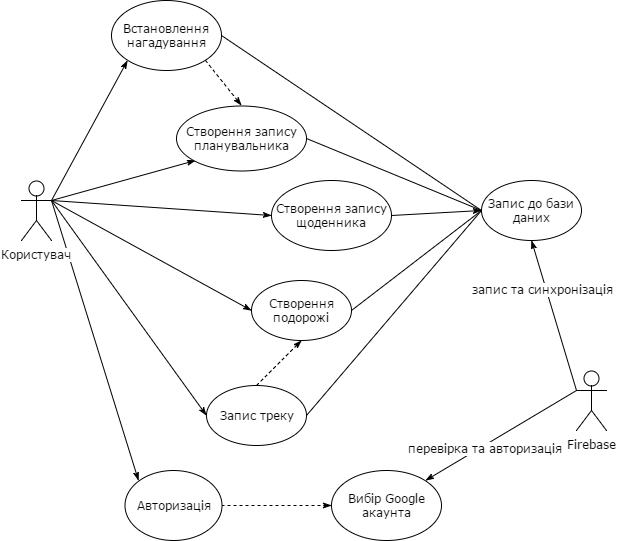
\includegraphics[width=1\textwidth]{02_diagram_usecase}
	\caption{Діаграма прецедентів механізму роботи з додатком}
	\label{diagram:usecase}
\end{figure}

\newpage
Користувач повинен мати можливість авторизуватися в додатку за~допомогою акаунта Google. Після вибору акаунта користувачем, Firebase перевіряє дані та відбувається авторизація користувача. Також, користувач повинен мати змогу створювати подорожі, записи щоденника та планувальника. Для створених записів планувальника повинна бути можливість встановлювати нагадування. Для подорожей користувач повинен мати можливість записувати трек переміщень. Всі дані зберігаються до бази даних та синхронізуються з допомогою Firebase.

%% TODO хоч я і паршиво для керівника дипломної роботи знаю ці діаграми, але факт, що акторами повинні бути лише зовнішні щодо розроблюваної системи чинники я все-таки знаю точно. До такого ТОЧНО ПРИЧЕПЛЯТЬСЯ. Якщо точно-точно нема користувачів з різними правами доступу щоб робити їх різними акторами, то, мабуть, треба зробити іншими акторами звернення до сторонніх систем... Хоча це краще ще десь уточнити.

\subsection{Формування та аналіз вимог до щоденника  під Android за допомогою діаграми діяльності}

\begin{figure}[H]
	\centering
	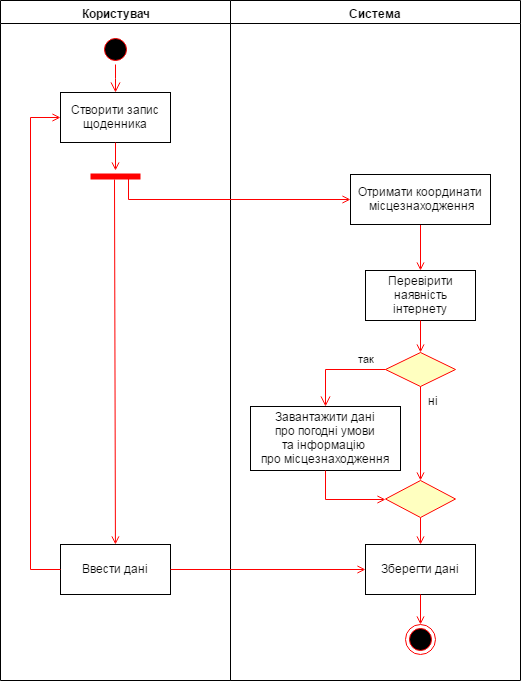
\includegraphics[width=0.6\textwidth]{02_diagram_activity-1}
	\caption{Діаграма діяльності механізму створення запису щоденника}
	\label{diagram:activity_diary}
\end{figure}

В процес створення запису щоденника залучений як користувач, так і~система. Після того, як користувач вирішує створити новий запис, система отримує координати місцезнаходження користувача, та, при наявності інтернет з'єднання, завантажує інформацію про місцезнаходження та дані про погодні умови в цьому місці. Після введення користувачем потрібних йому даних, та завершення створення запису, дані зберігаються. Для діаграми діяльності створення нового запису щоденника~див.~рис.~\ref{diagram:activity_diary}.

Для того, щоб встановити нагадування користувач повинен обрати його тип. При виборі нагадування за часом потрібно встановити час, в який це нагадування повинне спрацювати, а при виборі нагадування за місцем, користувач обирає місце на карті. Після цього інформація про нагадування зберігається та встановлюються будильники в системі. Діаграму діяльності механізму встановлення нагадування зображено на рис. \ref{diagram:activity_reminder}.

\begin{figure}[H]
	\centering
	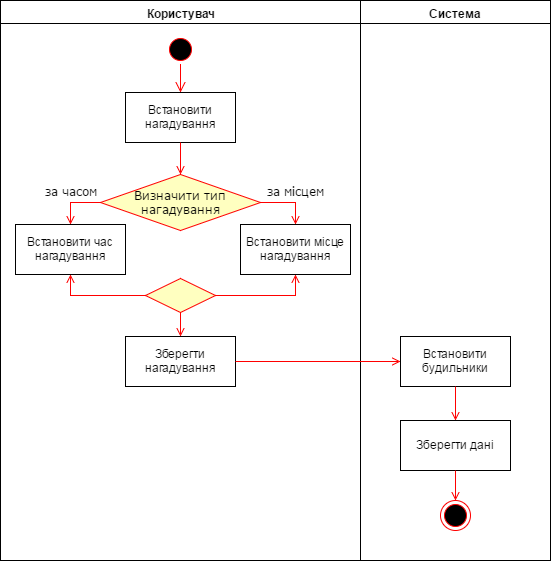
\includegraphics[width=0.7\textwidth]{02_diagram_activity-2}
	\caption{Діаграма діяльності механізму встановлення нагадування}
	\label{diagram:activity_reminder}
\end{figure}

Після того, як користувач почав запис треку система перевіряє його місцезнаходження. Якщо воно змінилося то відбувається збереження координат. Запис треку переміщень відбувається доти, доки користувач не завершить цей процес. Діаграму діяльності механізму запису треку переміщень подано на рис. \ref{diagram:activity_tracking}.

\begin{figure}[H]
	\centering
	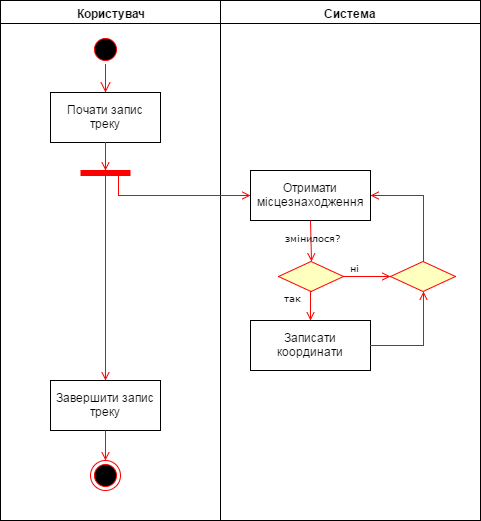
\includegraphics[width=0.7\textwidth]{02_diagram_activity-3}
	\caption{Діаграма діяльності механізму запису треку переміщень}
	\label{diagram:activity_tracking}
\end{figure}

\subsection{Аналіз вимог до Android-щоденника мандрівника за допомогою діаграми послідовності}
На базі отриманих даних, і заради детальнішого моделювання були розроблені діаграми послідовності для процесу створення запису планувальника та встановлення нагадування та для процесу створення запису щоденника.

На діаграмі послідовності об’єкт зображується у вигляді прямокутника на вершині пунктирної вертикальної лінії. Ця вертикальна лінія називається лінією життя об’єкту. Вона є фрагментом життєвого циклу об’єкту в процесі взаємодії. Кожне повідомлення представляється у вигляді стрілки між лініями життя двох об’єктів. Повідомлення з’являються в тому порядку, як вони показані на діаграмі (зверху вниз). Кожне повідомлення може бути позначене ім’ям.

\begin{figure}[H]
	\centering
	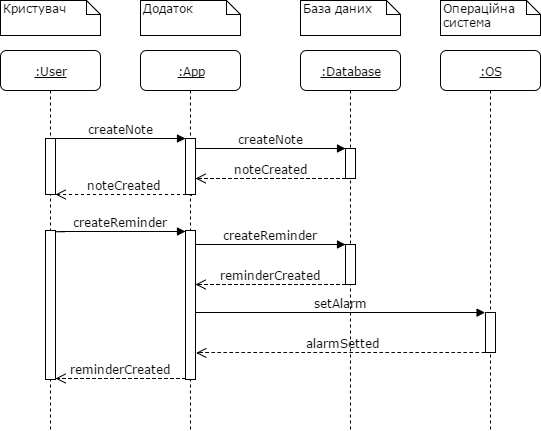
\includegraphics[width=0.85\textwidth]{02_diagram_sequence-1}
	\caption{Діаграма послідовності створення запису планувальника та~встановлення нагадування} 
	\label{diagram:sequence_reminder}
\end{figure}

Як видно з діаграми послідовності (див. рис. \ref{diagram:sequence_reminder}), після створення нагадування, дані записуються до бази даних та відбувається встановлення будильників у системі. 

\begin{figure}[H]
	\centering
	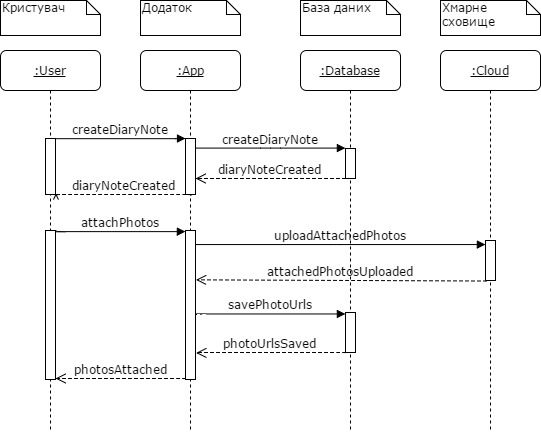
\includegraphics[width=0.85\textwidth]{02_diagram_sequence-2}
	\caption{Діаграма послідовності створення запису щоденника}
	\label{diagram:sequence_diary}
\end{figure}

Користувач також може додавати зображення до записів щоденника. Після вибору зображень, вони вивантажуються до хмарного сховища та відбувається збереження посилань до бази даних. Для детальної діаграми послідовності створення запису щоденника див. рис. \ref{diagram:sequence_diary}.

\subsection{Аналіз вимог до щоденника для мандрівників під Android за допомогою діаграми комунікації}
Діаграми комунікації відображають взаємодію ролей або об'єктів у~процесі функціонування системи, описують обмін даними (повідомленнями) між різними учасниками взаємодії. Такі діаграми моделюють сценарії поведінки системи~\cite{diploma_guidelines}. 

Діаграма комунікації для процесу перегляду подорожі та створення запису щоденника зображена на рис. \ref{diagram:communication}.

\begin{figure}[H]
	\centering
	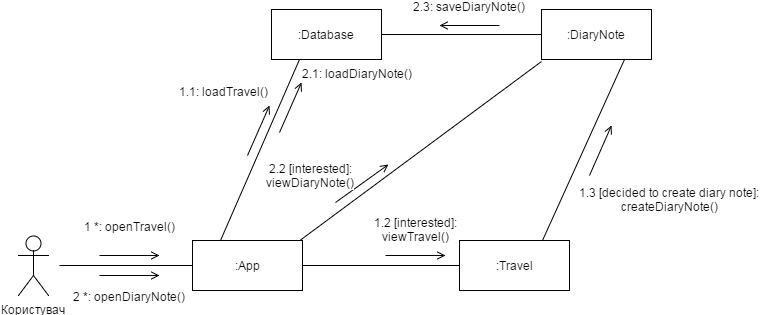
\includegraphics[width=1\textwidth]{02_diagram_communication}
	\caption{Діаграма комунікації для механізму перегляду подорожей та записів щоденника}
	\label{diagram:communication}
\end{figure}

При виборі користувачем подорожі чи запису щоденника, дані завантажуються з бази даних, та відображаються користувачеві. Також, знаходячись на екрані перегляду подорожі, користувач може вирішити створити запис щоденника для цієї подорожі.

\section{Архітектурне проектування Android-щоденника}
Формування архітектури – перший і основний крок у розв’язанні завдання проектування, що закладає фундамент уявлення програмної системи, здатної виконувати весь спектр детальних вимог~\cite{diploma_guidelines2}.

Створення архітектури – це проектування на найвищому рівні (логічна архітектура). Логічна архітектура описує систему в термінах її~принципової організації у вигляді пакетів, програмних класів і підсистем. Вона називається логічною, оскільки не визначає способи розгортання цих елементів у різних операційних системах або на фізичних комп’ютерах в~мережі (це відноситься до архітектури розгортання)~\cite{diploma_guidelines}.

Система Android надає різнобічну платформу додатків, на основі якої можна створювати інноваційні програми та ігри для мобільних пристроїв в~середовищі мови Java. Важливо знати наступні основні концепції, що~стосуються платформи додатків Android.

Додатки мають кілька точок входу.
Додатки для Android будуються з окремих компонентів, які можна викликати незалежно один від одного. Наприклад, окрема активність надає один екран для користувацького інтерфейсу, а служба незалежно виконує роботу у~фоновому режимі.

За допомогою об'єкта Intent з одного компонента можна запустити інший. Також можна запустити компонент з іншої програми, наприклад, активність з картографічного додатка, щоб показати адресу. Ця модель формує кілька точок входу для однієї програми, і при цьому користувач може вибрати будь-який додаток за замовчуванням для виконання тієї чи~іншої дії, яка може викликати інші додатки.

Додатки адаптуються до різних пристроїв.
Android надає адаптивну платформу додатків, яка дозволяє забезпечувати унікальні ресурси для різних конфігурацій пристроїв. Наприклад, можна створити різні файли \mbox{XML-макета} для екранів різних розмірів, а система буде визначати, який макет використовувати, з урахуванням розміру екрану даного пристрою.

Якщо якимось функціям програми потрібне певне обладнання, наприклад камера, можна запитувати його наявність в пристрої під час виконання. При необхідності також можна оголошувати функції, які потрібні додатку, для того, щоб такі магазини додатків, як Google Play, не~дозволяли встановлювати додатки на пристроях, в яких цих функцій немає~\cite{android_4}.

\subsection{Побудова діаграми пакетів для Android-щоденника}
Одним з важливих етапів архітектурного проектування є побудова діаграми пакетів. Діаграма пакетів є діаграмою, яка містить пакети класів і~залежності між ними. Вона описує архітектурну основу системи та~допомагає в управлінні масштабами й складністю системи. 

\begin{figure}[h]
	\centering
	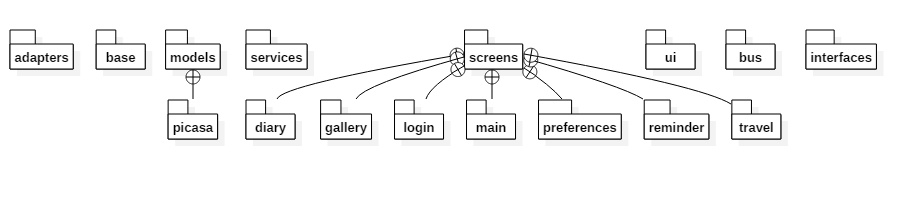
\includegraphics[width=1\textwidth]{diagram_packages}
	\caption{Діаграма пакетів для Android-щоденника}
	\label{diagram:packages}
\end{figure}

%«»

Пакет «adapters» призначений для адаптерів. Адаптер -- це об'єкт, що~діє як міст між представленням (view) і даними для цього представлення. Він забезпечує доступ до елементів даних. Також, адаптер відповідальний за~подання представлення для кожного елемента в наборі даних~\cite{adapter}. 

В пакеті «base» будуть знаходитися базові класи активностей, фрагментів чи інших компонентів.
Пакет «models» буде містити класи моделей, що необхідні для взаємодії з базою даних чи іншими службами. У пакеті «services» будуть міститися Android сервіси, тобто ті класи, що наслідуються від класу «Service» чи «IntentService».

Пакет «screens» призначений для різних екранів додатку, тому в ньому містяться пакети, що відповідають за конкретний екран додатку. Так, пакет «diary» буде містити активності та фрагменти, що відповідають за перегляд запису щоденника. Пакет «gallery» буде містити компоненти, що відповідають за перегляд галереї зображень при додаванні їх до запису щоденника. В пакеті «login» будуть знаходитися активності та фрагменти, що призначені для екрану авторизації користувача. Пакет «main» призначений для головного екрану додатка. В пакеті «reminder» будуть знаходитися активності та фрагменти, що відповідають за екран запису планувальника, а пакет «travel» буде містити те, що пов'язано з екраном подорожей.

Пакет «ui» буде містити додаткові компоненти інтерфейсу користувача, а пакет «interfaces» -- Java-інтерфейси. Для детальної діаграми пакетів додатка~див.~рис.~\ref{diagram:packages}.

%В пакеті «models» будуть знаходитися класи моделей, що необхідні для взаємодії з базою даних чи іншими сервісами. Пакет «screens» призначений для класів активностей, що являють собою окремі екрани додатку, тому в~нього були додані додаткові пакети, щоб розділити екрани по областях, за~які вони відповідають. Пакет «services» буде містити служби, а пакети «ui», «bus» та «interfaces» -- компоненти, що відповідають за інтерфейс користувача, шину подій та Java інтерфейси відповідно. Для детальної діаграми пакетів додатка~див.~рис.~\ref{diagram:packages}.

\subsection{Побудова діаграми компонентів Android-щоденника мандрівника}
Ще одним будівельним блоком для створення архітектури \mbox{об'єктно-орієнтованої} системи вважається компонент. Діаграма компонентів показує розбиття програмної системи на структурні компоненти та залежності між компонентами. В якості фізичних компонентів можуть бути файли, бібліотеки, модулі, виконувані файли, пакети і т.п. У багатьох середовищах розробки модуль або компонент відповідає файлу. Стрілки, що з'єднують модулі, показують відносини взаємозалежності аналогічні тим, які мають місце при компіляції вихідних текстів програм. Основними графічними елементами діаграми компонентів є компоненти, інтерфейси й залежності між ними. 

Клас «Application» є базовим класом для підтримки глобального стану програми. Для того, щоб надати йому власну реалізацію, потрібно створити підклас і вказати його повне ім'я в файлі маніфесту. В нашому випадку таким підкласом є «App». Він створюється в першу чергу, до того, як процес для додатка/пакета створиться.

Всі активності наслідуються від базового класу «AppCompatActivity», а ті, яким потрібна однакова базова логіка наслідуються від класу «BaseActivity». Всі фрагменти наслідуються від базового класу «Fragment».

Сервіс, що відповідає за запис треку переміщень наслідується від класу «Service», тому що він має працювати, доки користувач не зупинить запис. Інші сервіси додатку заслідуються від класу «IntentService». Всі сервіси мають бути вказані в файлі маніфесту. Детальну структуру компонентів додатку зображено на рис. \ref{diagram:hierarchy}.
%  (стор.~\pageref{diagram:hierarchy})

% \begin{figure}[H] % TODO думаю, тут все-таки краще спочатку пустити далі текст, далі розмістити рисунок. Дозволяє позбутися надто великих вертикальних дірок, вимогами розд.6.4 цілком допускається, і насправді активно використовується у практиці верстки взагалі.
\begin{figure}[H]
	\centering
	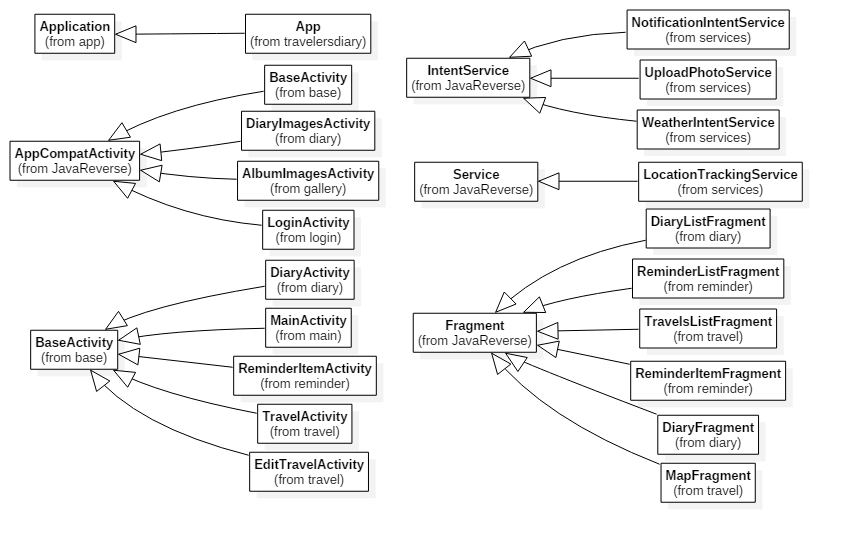
\includegraphics[width=1\textwidth]{02_diagram_hierarchy-1}
	\caption{Діаграма компонентів Android-щоденника}
	\label{diagram:hierarchy}
\end{figure}

\section{Детальне проектування Android-щоденника мандрівника}

Діаграма класів призначена для надання статичної структури моделі системи в термінології класів об’єктно-орієнтованого програмування. Діаграма класів відображує різні взаємозв’язки між окремими сутностями предметної області, такими як об’єкти й підсистеми, а також описує їхню внутрішню структуру й типи відносин \cite{diploma_guidelines}. 

Діаграма класів для Android-щоденника мандрівника зображена~на~рис.~\ref{diagram:models}.

\begin{figure}[H]
	\centering
	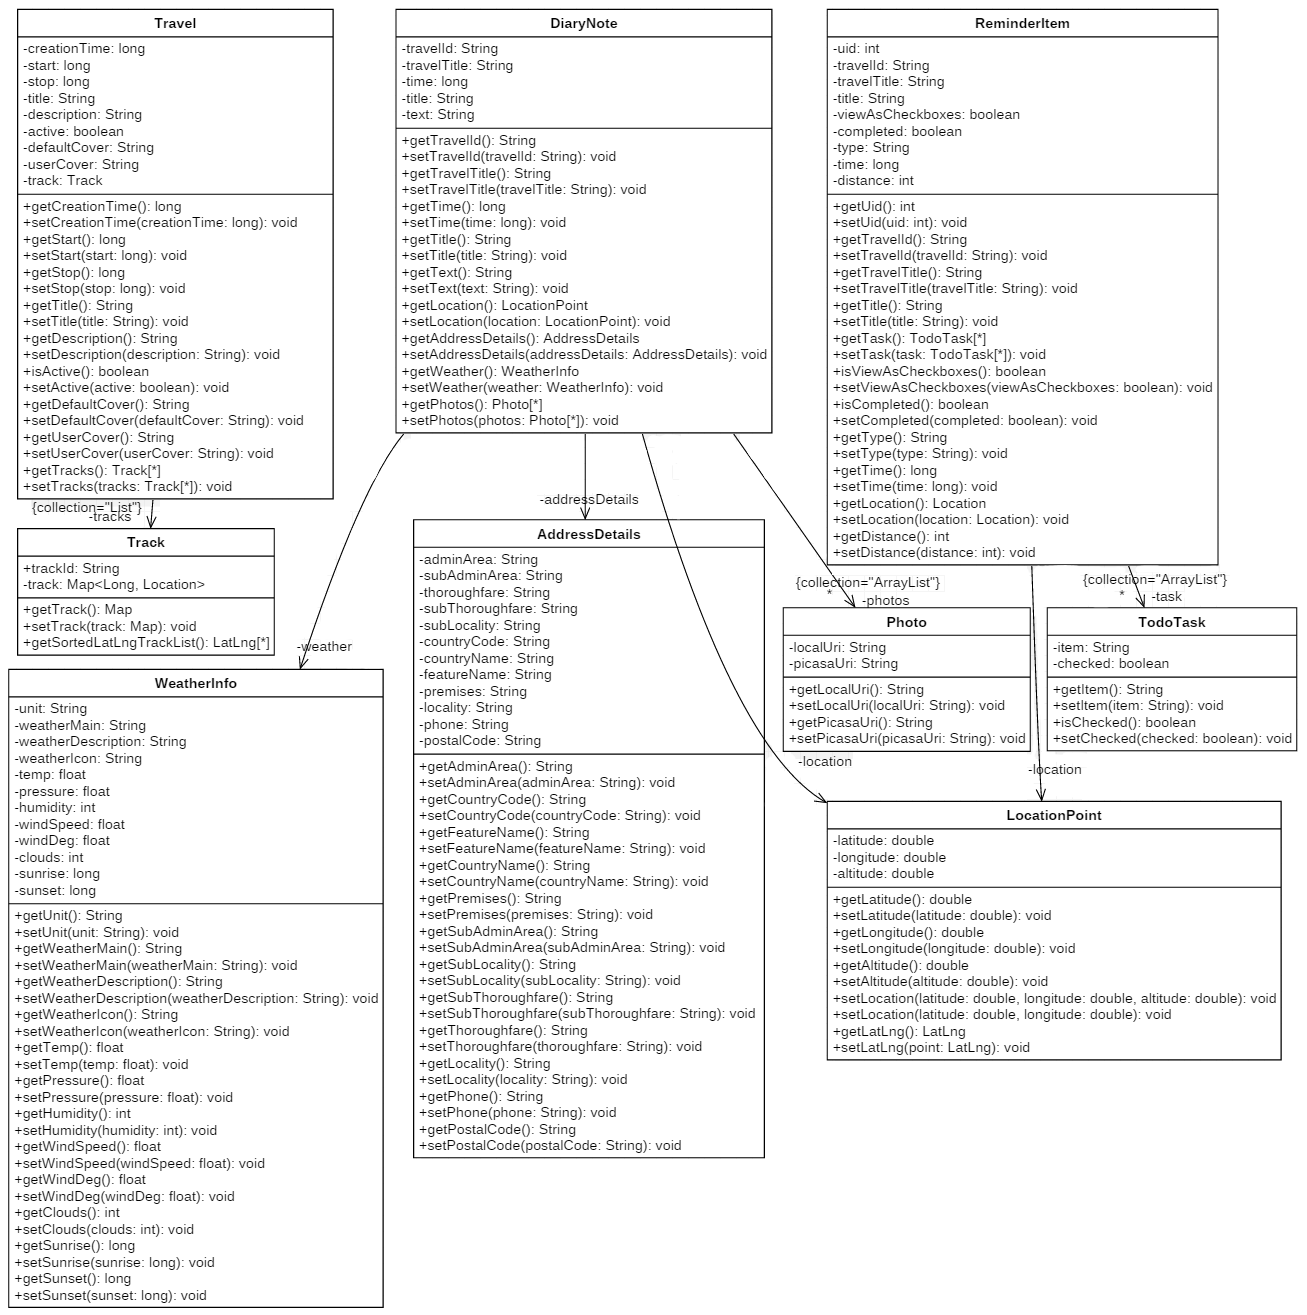
\includegraphics[width=1\textwidth]{02_diagram_models}
	\caption{Діаграма класів Android-щоденника}
	\label{diagram:models}
\end{figure}

Для подорожі було створено клас «Travel». Він міститиме назву та опис, час створення, початку та завершення подорожі, а також індикатор, який вказує активна вона чи ні. Додатково будуть поля для обкладинки подорожі.

У класі запису щоденника «DiaryNote» буде міститися назва, текст та час створення запису. Також, запис щоденника повинен мати список фото та інформацію про погодні умови й місце створення запису. Клас запису планувальника «ReminderItem» буде мати назву та текст, відмітку про виконання, а також інформацію про нагадування, таку як час чи координати нагадування та дистанція.

Для збереження інформації про погоду було створено клас «WeatherInfo», який буде містити інформацію про погодні умови, таку як температура, швидкість вітру, хмартність та інші погодні параметри. Для збереження інформації про місцезнаходження для запису щоденника, було створено клас «AdressDetails», що буде містити назву країни, міста, вулиці та інші відомості про місце.

Для запису треку переміщень необхідно зберігати координати місцезнаходження користувача. Для цього було створено клас «Track», що буде містити мапу, ключем в якій є час, а значенням -- координати користувача.

\section{Розгортання програмної системи для мандрівників на апаратних засобах}
Оскільки при розробці викорисловувалися сервіси Firebase, система може бути розгорнута під будь-яку платформу, що підтримує Firebase (Web, iOS, Unity та ін.). За темою роботи проводилася розробка Android клієнту. Діаграму розгортання системи представлено на рис. \ref{diagram:deployment}.

Для функціонування додатку необхідна операційна система Android версії 4.2 (API 16) і вище.

\begin{figure}[H]
	\centering
	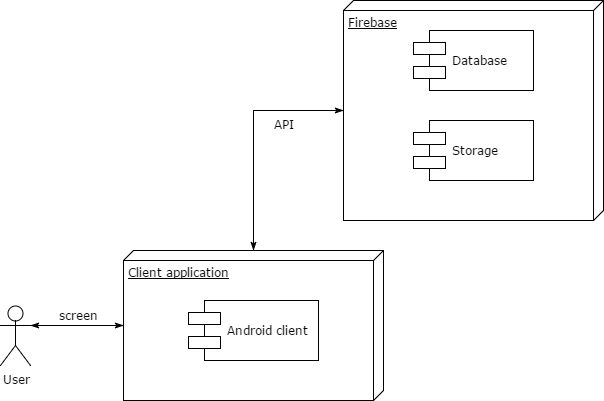
\includegraphics[width=0.8\textwidth]{diagram_deployment}
	\caption{Діаграма розгортання системи}
	\label{diagram:deployment}
\end{figure}

\section{Висновки до другого розділу}

У цьому розділі було сформовано вимоги до Android-щоденника на~основі результатів аналізу існуючих програмних продуктів. На основі сформованих вимог було побудовано діаграму прецедентів та визначено  детальні вимоги. Детальні вимоги відображають функції, якими необхідно наділити систему для забезпечення повного функціонування.

Також, було проведено аналіз вимог за допомогою діаграм діяльності, послідовності та комунікації, які допомагають отримати додаткове уявлення про сформовані вимоги.

Результатом роботи над даним розділом є формування та створення архітектури, що є основними кроками у розв'занні завдання проектування. Вони закладають фундамент програмної системи, описують систему в~термінах її принципової організації у вигляді пакетів, програмних класів і~підсистем.

\newpage
Також, було проаналізовано основні концепції платформи Android додатків. Було побудовано діаграму пакетів, на якій відображено пакети та зв'язки між ними, та діаграму компонентів, яка показує розбиття програмної системи на структурні компоненти та залежності між ними.

Проведено детальне проектування системи, створено діаграму взаємодії активностей додатку та діаграму моделей. Також описано розгортання системи на апаратних засобах, розроблено схему розгортання та описано необхідні засоби для функціонування додатку.

\end{document}